\section{Spectre}

Spectrul reprezintă un ansamblu discret sau continuu de valori care pot fi
luate de o anumită mărime. În particular, componentele monocromatice ale unei
radiații electromagnetice.

Spectroscopul este un instrument care descompune radiația electromagnetică
complexă în componentele monocromatice, utilizat pentru studiul spectrelor.

\subsection{Spectroscopul cu prismă}

În componența unui aparat spectral intră un dispozitiv ce descompune radiația
emisă în radiațiile monocromatice componente.

În spectroscopul cu prismă, această sarcină o are prisma optică, pe baza
fenomenului de dispersie.

\begin{wrapfigure}{r}{0.51\textwidth}
    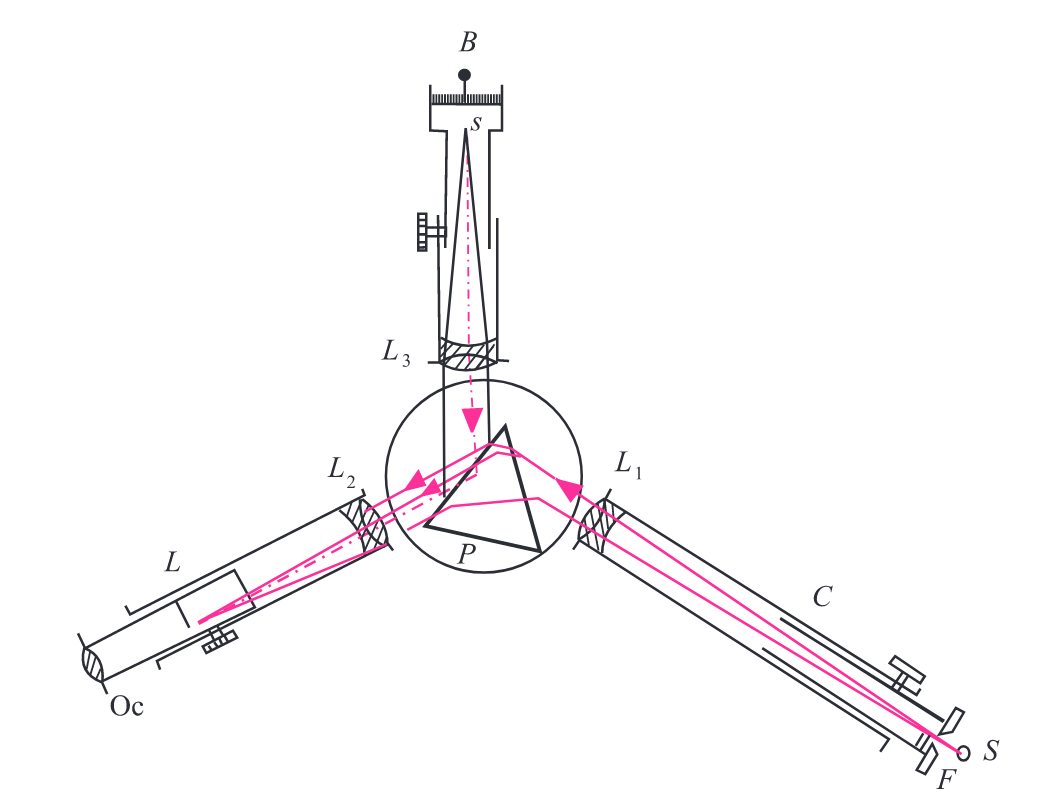
\includegraphics[width=0.5\textwidth]{fig/spectroscop}
    \caption{Schema spectroscopului}
\end{wrapfigure}

Spectroscopul cu prismă are în componență un tub $C$, numit \emph{colimator},
prevăzut cu o fantă $F$ aflată în focarul unui sistem optic convergent $L_1$.
Sursa $S$ emite raze divergente, ce trec prin $F$ și sunt transformate într-un
fascicul paralel de către $L_1$.

Prisma optică $P$ va dispersa radiațiile incidente sub diferite unghiuri,
fasciculele urmând să fie focalizate de obiectivul $L_2$ de la capătul lunetei
$L$, în planul focal al obiectivului.

În ocularul lunetei intră și fasciculul de lumină reflectat pe fața prismei,
provenit de la un alt colimator, ce proiectează imaginea unei riglete
micrometrice $s$, iluminată de becul $B$.

Imaginile fantei corespunzătoare radiații monocromatice reprezintă liniile
spectrale observate prin intermediul ocularului, ce are rol de lupă.

Dacă în planul focal al obiectivului $L_2$ se așază o placă fotografică,
aparatul spectral poartă denumirea de \emph{spectograf}.

Într-un aparat spectral, prisma și lentilele sunt din sticlă pentru domeniul
vizibil, din cuarț pentru ultraviolet, și din materiale transparente, precum
monocristalul din clorură de sodiu, pentru infraroșu.

Spectrele pot fi: \emph{continue} sau \emph{discontinue}.

Setul de lungimi de undă de diferite lungimi de undă se împarte în
\emph{spectre de emisie} și \emph{spectre de absorbție}.

Spectrele de emisie caracterizează substanța emițătoare de lumină, iar cele de
absorbție, substanță absorbantă.

În funcție de natura sursei emitente, spectrele de emisie pot fi continue, sau discontinue de linii sau de bandă.

În funcție de sistemul de particule studiat, spectrele pot fi atomice sau moleculare.

\subsubsection{Spectre continue de emisie}

Lumina emisă de toate corpurile solide și lichide incandescente, precum
filamentul unui bec, un cărbune, sau metalul topit, conține o multitudine de
radiații spectrale suprapuse, cu lungimi de undă foarte apropiate.

Corpurile solide sau lichide, aduse la incandescență, emit un spectru continuu de culori: roșu, portocaliu, galben, verde, albastru, indigo, violet.

De exemplu, filamentul de wolfram al unui bec emite o lumină de culoare
diferită în funcție de temperatură. La 700$^\circ$C emite roșu închis, la
1000$^\circ$C roșu aprins, la 1200$^\circ$C portocaliu, la 1300$^\circ$C alb,
și la 1400$^\circ$C alb strălucitor. La fel și în cazul stelelor, clasificate
în funcție de culoare, care depinde de temperatură.

\subsubsection{Spectre discontinue de emisie}

Spectrele discontinue sunt emise de gazele din tuburile de descărcare (vapori
de mercur, sodiu, potasiu). Acestea pot fi spectre de linii sau spectre de
bandã.

Spectrele de linii sunt emise de substanțele gazoase aflate în stare atomică,
și iau forma unor linii strălucitoare de diferite culori, pe un fond negru.

Spectrele de bandă sunt asemănătoare spectrelor de linii, însă liniile sunt
grupate în benzi. Sunt emise de substanțele gazoase aflate în stare moleculară
($H_2$, $O_2$, $N_2$).

Înmuind un fir de platină într-o soluție NaCl și introducându-l în flacăra unui
bec Bunsen, flacăra va lua aspectul caracteristic fiecărui metal: galben pentru
natriu, roșu purpuriu pentru potasiu etc.

\subsubsection{Spectre de absorbție}

Dacă un spectru continuu traversează un gaz la o temperatură mai joasă decât
temperatura sursei, o soluție lichidă, sau o sticlă colorată, se obține un
spectru de absorbție. Acesta se reprezintă ca un spectru continuu brăzdat de
lini sau benzi întunecate.

Culoarea unei substanțe transparente este dată de suprapunerea radiațiilor
neabsorbite.

De exemplu, prin macerarea frunzelor de spanac în alcool sau acetonă și
filtrarea lichidului rezultat, se obține o soluție ce conține clorofilă.
Spectrul de absorbție prezintă bezi întunecate în domeniul roșu, albastru, și
violet. Radiațiile din centrul spectrului sunt mai puțin absorbite, determinând
culoarea verde a clorofilei.

Studiind spectrele de emisie și de absorbție, Kirchhoff a determinat legea:
\emph{fiecare substanță absoarbe acele radiații pe care le poate emite în
aceleași condiții de temperatură și presiune.}

Fiecare atom, ion, sau moleculă are un spectru de emisie și de absorbție
caracteristic.

Liniile întunecate din spectrul solar corespund elementelor aflate în coroana
solară, și care absorb radiațiile emise din interiorul stelei.

\clearpage

Spectrele atomice mai pot fi împărțite în:
\begin{itemize}
    \item \emph{spectre optice} -- tranzițiile electronilor de valență din
        atom. Conțin radiații din domeniul vizibil, ultraviolet, și infraroșu.
        Orice element chimic este caracterizat de un spectru de emisie format
        dintr-o succesiune de linii spectrale. Fiecare linie spectrală apare ca
        rezultat al tranziției radiative a atomului de pe un nivel energetic
        superior, de energie $E_i$, pe un nivel energetic inferior, de energie
        $E_f$.
    \item \emph{spectre de radiații X} -- Excitarea electronilor din păturile
        interioare ale atomilor necesită o energie mult mai mare decât a electronilor din păturile exterioare. Trecerea acestor electroni din starea excitată în starea fundamentală determină emiterea radiațiilor X, cu lungimi de undă foarte mici.
\end{itemize}
